
\documentclass[letterpaper,hide notes,xcolor={table,svgnames},pdftex,10pt]{beamer}
\def\showexamples{t}


%\usepackage[svgnames]{xcolor}

%% Demo talk
%\documentclass[letterpaper,notes=show]{beamer}

\usecolortheme{crane}
\setbeamertemplate{navigation symbols}{}

\usetheme{MyPittsburgh}
%\usetheme{Frankfurt}

%\usepackage{tipa}

\usepackage{hyperref}
\usepackage{graphicx,xspace}
\usepackage[normalem]{ulem}
\usepackage{multicol}
\usepackage{amsmath,amssymb,amsthm,graphicx,xspace}
\newcommand\SF[1]{$\bigstar$\footnote{SF: #1}}

\usepackage[default]{sourcesanspro}
\usepackage[T1]{fontenc}
\usepackage[scaled]{beramono}
\usepackage{tikzpagenodes}

\newcounter{tmpnumSlide}
\newcounter{tmpnumNote}


% old question code
%\newcommand\question[1]{{$\bigstar$ \small \onlySlide{2}{#1}}}
% \newcommand\nquestion[1]{\ifdefined \presentationonly \textcircled{?} \fi \note{\par{\Large \textbf{?}} #1}}
% \newcommand\nanswer[1]{\note{\par{\Large \textbf{A}} #1}}


 \newcommand\mnote[1]{%
   \addtocounter{tmpnumSlide}{1}
   \ifdefined\showcues {~\tiny\fbox{\arabic{tmpnumSlide}}}\fi
   \note{\setlength{\parskip}{1ex}\addtocounter{tmpnumNote}{1}\textbf{\Large \arabic{tmpnumNote}:} {#1\par}}}

\newcommand\mmnote[1]{\note{\setlength{\parskip}{1ex}#1\par}}

%\newcommand\mnote[2][]{\ifdefined\handoutwithnotes {~\tiny\fbox{#1}}\fi
% \note{\setlength{\parskip}{1ex}\textbf{\Large #1:} #2\par}}

%\newcommand\mnote[2][]{{\tiny\fbox{#1}} \note{\setlength{\parskip}{1ex}\textbf{\Large #1:} #2\par}}

\newcommand\mquestion[2]{{~\color{red}\fbox{?}}\note{\setlength{\parskip}{1ex}\par{\Large \textbf{?}} #1} \note{\setlength{\parskip}{1ex}\par{\Large \textbf{A}} #2\par}\ifdefined \presentationonly \pause \fi}

\newcommand\blackboard[1]{%
\ifdefined   \showblackboard
  {#1}
  \else {\begin{center} \fbox{\colorbox{blue!30}{%
         \begin{minipage}{.95\linewidth}%
           \hspace{\stretch{1}} Some space intentionally left blank; done at the blackboard.%
         \end{minipage}}}\end{center}}%
         \fi%
}



%\newcommand\q{\tikz \node[thick,color=black,shape=circle]{?};}
%\newcommand\q{\ifdefined \presentationonly \textcircled{?} \fi}

\usepackage{listings}
\lstset{basicstyle=\footnotesize\ttfamily,
	breaklines=true,
	aboveskip=15pt,
  	belowskip=15pt,
	frame=lines,
	numbers=left, basicstyle=\scriptsize, numberstyle=\tiny, stepnumber=0, numbersep=2pt
}

\usepackage{siunitx}
\newcommand\sius[1]{\num[group-separator = {,}]{#1}\si{\micro\second}}
\newcommand\sims[1]{\num[group-separator = {,}]{#1}\si{\milli\second}}
\newcommand\sins[1]{\num[group-separator = {,}]{#1}\si{\nano\second}}
\sisetup{group-separator = {,}, group-digits = true}

%% -------------------- tikz --------------------
\usepackage{tikz}
\usetikzlibrary{positioning}
\usetikzlibrary{arrows,backgrounds,automata,decorations.shapes,decorations.pathmorphing,decorations.markings,decorations.text,decorations.pathreplacing}

\tikzstyle{place}=[circle,draw=blue!50,fill=blue!20,thick, inner sep=0pt,minimum size=6mm]
\tikzstyle{transition}=[rectangle,draw=black!50,fill=black!20,thick, inner sep=0pt,minimum size=4mm]

\tikzstyle{block}=[rectangle,draw=black, thick, inner sep=5pt]
\tikzstyle{bullet}=[circle,draw=black, fill=black, thin, inner sep=2pt]

\tikzstyle{pre}=[<-,shorten <=1pt,>=stealth',semithick]
\tikzstyle{post}=[->,shorten >=1pt,>=stealth',semithick]
\tikzstyle{bi}=[<->,shorten >=1pt,shorten <=1pt, >=stealth',semithick]

\tikzstyle{mut}=[-,>=stealth',semithick]

\tikzstyle{treereset}=[dashed,->, shorten >=1pt,>=stealth',thin]

\usepackage{ifmtarg}
\usepackage{xifthen}
\makeatletter
% new counter to now which frame it is within the sequence
\newcounter{multiframecounter}
% initialize buffer for previously used frame title
\gdef\lastframetitle{\textit{undefined}}
% new environment for a multi-frame
\newenvironment{multiframe}[1][]{%
\ifthenelse{\isempty{#1}}{%
% if no frame title was set via optional parameter,
% only increase sequence counter by 1
\addtocounter{multiframecounter}{1}%
}{%
% new frame title has been provided, thus
% reset sequence counter to 1 and buffer frame title for later use
\setcounter{multiframecounter}{1}%
\gdef\lastframetitle{#1}%
}%
% start conventional frame environment and
% automatically set frame title followed by sequence counter
\begin{frame}%
\frametitle{\lastframetitle~{\normalfont(\arabic{multiframecounter})}}%
}{%
\end{frame}%
}
\makeatother

\makeatletter
\newdimen\tu@tmpa%
\newdimen\ydiffl%
\newdimen\xdiffl%
\newcommand\ydiff[2]{%
    \coordinate (tmpnamea) at (#1);%
    \coordinate (tmpnameb) at (#2);%
    \pgfextracty{\tu@tmpa}{\pgfpointanchor{tmpnamea}{center}}%
    \pgfextracty{\ydiffl}{\pgfpointanchor{tmpnameb}{center}}%
    \advance\ydiffl by -\tu@tmpa%
}
\newcommand\xdiff[2]{%
    \coordinate (tmpnamea) at (#1);%
    \coordinate (tmpnameb) at (#2);%
    \pgfextractx{\tu@tmpa}{\pgfpointanchor{tmpnamea}{center}}%
    \pgfextractx{\xdiffl}{\pgfpointanchor{tmpnameb}{center}}%
    \advance\xdiffl by -\tu@tmpa%
}
\makeatother
\newcommand{\copyrightbox}[3][r]{%
\begin{tikzpicture}%
\node[inner sep=0pt,minimum size=2em](ciimage){#2};
\usefont{OT1}{phv}{n}{n}\fontsize{4}{4}\selectfont
\ydiff{ciimage.south}{ciimage.north}
\xdiff{ciimage.west}{ciimage.east}
\ifthenelse{\equal{#1}{r}}{%
\node[inner sep=0pt,right=1ex of ciimage.south east,anchor=north west,rotate=90]%
{\raggedleft\color{black!50}\parbox{\the\ydiffl}{\raggedright{}#3}};%
}{%
\ifthenelse{\equal{#1}{l}}{%
\node[inner sep=0pt,right=1ex of ciimage.south west,anchor=south west,rotate=90]%
{\raggedleft\color{black!50}\parbox{\the\ydiffl}{\raggedright{}#3}};%
}{%
\node[inner sep=0pt,below=1ex of ciimage.south west,anchor=north west]%
{\raggedleft\color{black!50}\parbox{\the\xdiffl}{\raggedright{}#3}};%
}
}
\end{tikzpicture}
}


%% --------------------

%\usepackage[excludeor]{everyhook}
%\PushPreHook{par}{\setbox0=\lastbox\llap{MUH}}\box0}

%\vspace*{\stretch{1}

%\setbox0=\lastbox \llap{\textbullet\enskip}\box0}

\setlength{\parskip}{\fill}

\newcommand\noskips{\setlength{\parskip}{1ex}}
\newcommand\doskips{\setlength{\parskip}{\fill}}

\newcommand\xx{\par\vspace*{\stretch{1}}\par}
\newcommand\xxs{\par\vspace*{2ex}\par}
\newcommand\tuple[1]{\langle #1 \rangle}
\newcommand\code[1]{{\sf \footnotesize #1}}
\newcommand\ex[1]{\uline{Example:} \ifdefined \presentationonly \pause \fi
  \ifdefined\showexamples#1\xspace\else{\uline{\hspace*{2cm}}}\fi}

\newcommand\ceil[1]{\lceil #1 \rceil}


\AtBeginSection[]
{
   \begin{frame}
       \frametitle{Outline}
       \tableofcontents[currentsection]
   \end{frame}
}



\pgfdeclarelayer{edgelayer}
\pgfdeclarelayer{nodelayer}
\pgfsetlayers{edgelayer,nodelayer,main}

\tikzstyle{none}=[inner sep=0pt]
\tikzstyle{rn}=[circle,fill=Red,draw=Black,line width=0.8 pt]
\tikzstyle{gn}=[circle,fill=Lime,draw=Black,line width=0.8 pt]
\tikzstyle{yn}=[circle,fill=Yellow,draw=Black,line width=0.8 pt]
\tikzstyle{empty}=[circle,fill=White,draw=Black]
\tikzstyle{bw} = [rectangle, draw, fill=blue!20, 
    text width=4em, text centered, rounded corners, minimum height=2em]
    
    \newcommand{\CcNote}[1]{% longname
	This work is licensed under the \textit{Creative Commons #1 3.0 License}.%
}
\newcommand{\CcImageBy}[1]{%
	\includegraphics[scale=#1]{creative_commons/cc_by_30.pdf}%
}
\newcommand{\CcImageSa}[1]{%
	\includegraphics[scale=#1]{creative_commons/cc_sa_30.pdf}%
}
\newcommand{\CcImageNc}[1]{%
	\includegraphics[scale=#1]{creative_commons/cc_nc_30.pdf}%
}
\newcommand{\CcGroupBySa}[2]{% zoom, gap
	\CcImageBy{#1}\hspace*{#2}\CcImageNc{#1}\hspace*{#2}\CcImageSa{#1}%
}
\newcommand{\CcLongnameByNcSa}{Attribution-NonCommercial-ShareAlike}

\newenvironment{changemargin}[1]{% 
  \begin{list}{}{% 
    \setlength{\topsep}{0pt}% 
    \setlength{\leftmargin}{#1}% 
    \setlength{\rightmargin}{1em}
    \setlength{\listparindent}{\parindent}% 
    \setlength{\itemindent}{\parindent}% 
    \setlength{\parsep}{\parskip}% 
  }% 
  \item[]}{\end{list}} 




\title{Lecture 21 --- Laws of Performance \& Performance Culture }

\author{Jeff Zarnett \\ \small \texttt{jzarnett.uwaterloo.ca}}
\institute{Department of Electrical and Computer Engineering \\
  University of Waterloo}
\date{\today}


\begin{document}

\begin{frame}
  \titlepage

 \end{frame}


\part{Laws of Performant Software}

\begin{frame}
\partpage
\end{frame}


\begin{frame}
\frametitle{Laws of Performant Software}

Suppose you want to write fast programs...\\
\quad And you like checklists and handy rules. 

If so, you are in luck, because there is Crista's Five Laws of Performant Software!

\begin{center}
	
\includegraphics[width=0.5\textwidth]{images/thelaw.png}
\end{center}

\end{frame}



\begin{frame}
\frametitle{Rule 1: Knowledge is Power}

\textbf{1. Programming language $<<$ Programmers' awareness of performance.}

There is no programming language that is magic, whether good or evil. 

All the major programming languages allow you to write programs that perform well or badly. 

High level languages give you lots of options...\\
\quad Do I use an array? A vector? A list? 

What do they do behind the scenes?\\
\quad Is there a better way?

\end{frame}



\begin{frame}
\frametitle{Rule 1 Asterisk}

\begin{center}
	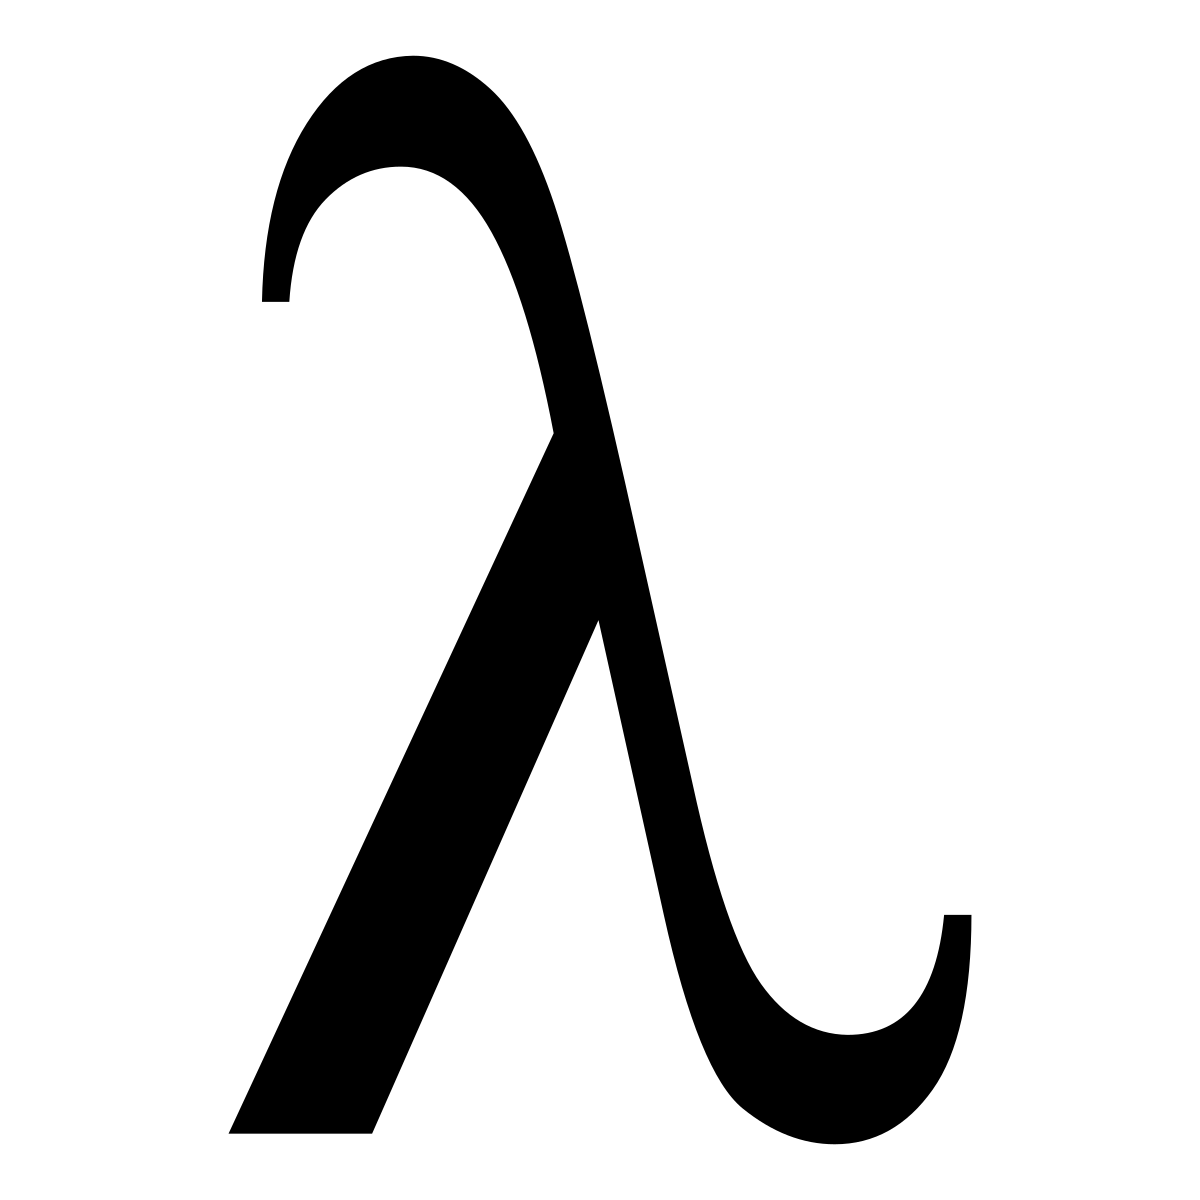
\includegraphics[width=0.2\textwidth]{images/lambda.png}
\end{center}

Some languages lend themselves better to parallelization than others. 

A language may force a certain way of thinking, based on its rules (e.g., functional programming languages). 

But there is no reason why the way of thinking can't be applied in another language.


\end{frame}



\begin{frame}
\frametitle{Rule 2: Nonlinear Output}

\textbf{2. $d(f^{\tau}(x), f^{\tau}(y)) > e^{\alpha\tau} d(x, y)$ or small details matter.}

If two versions of the code are $x$ and $y$, the difference between the performance outcomes $f(x), f(y)$ is much larger than the difference between the code.

Did you fix a memory leak? The addition of one \texttt{free()} call is a single line code change but can, in the long run, have a dramatic impact on performance. 

Don't overlook the small stuff!

\end{frame}




\begin{frame}
\frametitle{Rule 3: Establish Boundaries}

\textbf{3. corr(performance degradation, unbounded resource usage) > 0.9.}

There is a very high correlation between performance degradation and unbounded use of resources. 

Often times we focus on functionality: the software must have the following 847~251 features! 

But if you want a program that scales you need to think in terms of operation, not functionality.

\end{frame}



\begin{frame}
\frametitle{Rule 3: Establish Boundaries}

Resources need to be limited. 

If there aren't hard limits, eventually a resource will be exhausted. 

If the program starts threads, use a thread pool and the thread pool should have a fixed size. 

Is there a cache? It needs a maximum size. 

If you need to read input, don't use a function that reads an entire line (of arbitrary length). 

\end{frame}



\begin{frame}
\frametitle{Rule 3: Establish Boundaries}

Furthermore your program needs design effort given to what happens when resources are exceeded. 

So you decide to set a request queue size; once that queue is full, further requests are rejected in some well-understood manner. 


\end{frame}



\begin{frame}
\frametitle{Rule 4: Do Experiments}

\begin{center}
	
\includegraphics[width=0.3\textwidth]{images/ndg.jpg}
\end{center}

If you want your code to be faster you have to know why it is slow. 

It's okay not to know the answers, but not knowing how to find out is a problem. 

Don't guess; measure.

\end{frame}



\begin{frame}
\frametitle{Rule 5: You Can't Outrun the Fork}

\textbf{5. N*bad != good.}

No amount of nodes, cores, memory, etc, will save you from poorly-written code.

Throwing more hardware at the problem is expensive and ineffective in the long term. 

Bad code is still bad no matter how much hardware it runs on. 

\end{frame}

\part{Performance Tips}

\begin{frame}
\partpage
\end{frame}



\begin{frame}
\frametitle{Magnitude}

\textbf{Understand the order of magnitude that matters.} 

Perhaps you are writing code where 100 CPU cycles matters. 

If so, a function that will acquire a lock through some sort of shared-memory interlocked instruction then this instruction is performance murder. 

And it might be even worse if lock acquisition fails and you get blocked for 100~000 cycles trying to acquire the lock... 

On the other hand, if you have a network intensive code then 100 cycles do not matter even the smallest bit because it is lost in the noise of the network.

\end{frame}



\begin{frame}
\frametitle{Worst Case Scenario}

Plan for the worst case scenario (not the nuclear apocalypse).

You can end up paying many more orders of magnitude in cost than you expected under ordinary circumstances.

No doubt you have seen these sorts of things as well and it is an awful user experience. 

The spinning beach ball of death and the ``Not Responding'' added to the title bar are all symptoms of this situation. 


\end{frame}



\begin{frame}
\frametitle{Acknowledge Asynchrony}

A lot of things are asynchronous without declaring themselves to be.

\begin{center}
	
\includegraphics[width=0.5\textwidth]{images/patientbear.jpg}
\end{center}

\end{frame}



\begin{frame}
\frametitle{Acknowledge Asynchrony}

Suppose that Jordan is writing code to return a list of fonts to be used in the UI. 

The code checks a local font cache, and if that is already initialized, returns the fonts found in the cache in a List object. 

If the cache is not initialized, however, the data needs to be loaded, perhaps from the printer. 

Morgan intends to use this list of fonts in the UI of the program but is unaware that in certain circumstances this call will take much longer.

\end{frame}



\begin{frame}
\frametitle{Acknowledge Asynchrony}

Supposing that the API just returns a \texttt{List<Font>}, it is not obvious to Morgan where these come from. 

And in local testing on the dev machine with nothing on it and nothing else doing and the printer is always turned on.

Thus even if the cache is not initialized it is ``fast enough''. 

But in the real world, of course, the printer will be down and unicorns are nowhere to be found and it runs up against some hard timeout of 20 seconds. 

\end{frame}



\begin{frame}
\frametitle{Acknowledge Asynchrony}

If Jordan's API now has a return type of \texttt{Task<List>} then it is obvious to Morgan that there is something asynchronous going on here some of the time. 

With this information in hand, the UI won't wait for this task. 

We might even convince Jordan to give us partial results (so we can draw the UI elements as backing data arrives) or at the very least, a progress bar. 

Users love progress bars. 

They are wildly inaccurate and not super informative even if they are accurate, but at least they give the user the impression that something is happening.

\end{frame}

\part{Performance Culture}

\begin{frame}
\partpage
\end{frame}



\begin{frame}
\frametitle{Would you work for him?}

\begin{center}
	
\includegraphics[width=0.5\textwidth]{images/drevil.jpg}
\end{center}

\end{frame}


\begin{frame}
\frametitle{Performance Problem Check}

The author's recommendations of warning signs that performance culture is off the rails:

\begin{itemize}
\item Answering the question, ``how is the product doing on my key performance metrics,'' is difficult.
\item Performance often regresses and team members either don't know, don't care, or find out too late to act.
\item Blame is one of the most common responses to performance problems (either people, infrastructure, or both).
\end{itemize}

\end{frame}

\begin{frame}
\frametitle{Performance Problem Check}

The author's recommendations of warning signs that performance culture is off the rails:

\begin{itemize}

\item Performance tests swing wildly, cannot be trusted, and are generally ignored by most of the team.
\item Performance is something one, or a few, individuals are meant to keep an eye on, instead of the whole team.
\item Performance issues in production are common, and require ugly scrambles to address (and/or cannot be reproduced).
\end{itemize}

\end{frame}



\begin{frame}
\frametitle{Human After All}


As tempting as it is to say these are all technical issues, they are really human problems. 

It would obviously be preferable to start with a good performance culture in the first place, but that is not always going to happen. 

But suppose you are already in a hole. The usual course of action is to stop and say to yourself ``I appear to be in a hole... I know, I'll dig my way out!''. 

The right thing to do would be stop digging, of course...
\end{frame}



\begin{frame}
\frametitle{Change Comes From Within}

Change has to come from both the top down and the bottom up. 

Management needs to make performance a priority: ask questions, demand rigour... 

While at the same time, people doing the development need to understand the performance of what they write, making practice improvements. 

Both sides need to have zero tolerance for regression.

\end{frame}



\begin{frame}
\frametitle{Run, Run Away}

\begin{center}
	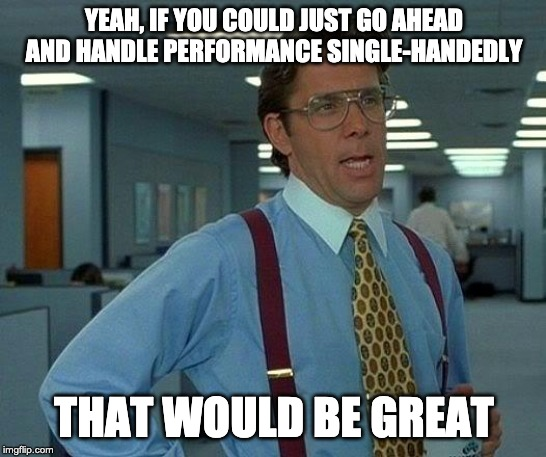
\includegraphics[width=0.6\textwidth]{images/wouldbegreat.jpg}
\end{center}

\end{frame}


\begin{frame}
\frametitle{There Can't Be One}

If only one person is responsible for performance, this will not work. One person could not reasonably keep up with the rest of the team. 

If the other developers don't have performance in mind when writing, it is a big waste of time for the performance person.

If this isn't convincing, think about unit tests. 

Could you really ``outsource'' the writing of all unit tests to one person? And would code quality be the same if you did?

\end{frame}



\begin{frame}
\frametitle{Management Matters}

Managers need to budget time, reward the work, and encourage performance work. 

Managers who don't understand performance culture are likely to be caught by surprise and blame things. 

Consider the story of Managers A and B (see the notes).

\end{frame}



\begin{frame}
\frametitle{Startup}


But this is a startup, you object, why does it matter, because we need the minimum viable product and we needed it yesterday.

And also, VCs like features. 

Well maybe, but architecture matters. 

There's time to fix things later, maybe, but you can really cripple your startup by choosing the wrong things early on. 

\end{frame}



\begin{frame}
\frametitle{Performance Tests}

After a discussion of the why and the what, it is time to think about how to make it systematic. 

If it is not systematic, it will not get done and it will be dropped when in a time crunch. And development teams are always in a time crunch! 

This is why best practices have automated unit tests that run on every commit. 

If something has significantly regressed performance, the build failed and the commit is no good. 

This obviously requires that the tests be meaningful, testing effectively and not overly noisy. 

\end{frame}



\begin{frame}
\frametitle{Performance Tests}

Performance tests may be a bit too large and difficult to run for every commit or every build. 

Although it would be nice to know exactly which commit is the cause of the problem, you may want a test that runs overnight to see the long term trends. 

And thus a 12-hour test is probably unsuitable for this. 

The solution is, obviously, levels of test. 

\end{frame}



\begin{frame}
\frametitle{Zero Tolerance}

A zero tolerance rules advocated: anything that significantly regresses performance is reverted and re-worked. 

No exceptions, no questions, no pleading one's case, etc. 

If exceptions are allowed, exceptions quickly become the rule, and promises to fix something later are procrastinated endlessly.

Obviously when code does more it should be expected to take longer, but then the test(s) should be adjusted as well.

\end{frame}



\begin{frame}
\frametitle{Metrics}

There are, roughly speaking, two categories of metrics:

\begin{itemize}
	\item \textit{Consumption}: measure resources consumed by running a test.
	\item \textit{Observational}: measure the outcomes of running the test, from the view of outside the system.
\end{itemize}


\end{frame}




\begin{frame}
\frametitle{Observational Metrics}

It might seem like observational metrics are all that we care about. 

End users care about the amount of time it takes to complete their work, or management/sales/marketing/C-levels care about the throughput and that's it. 

This matters, sure, but it's not enough to know the outcome; the consumption metrics are necessary to break down why the total time is what it is.

\end{frame}



\begin{frame}
\frametitle{Observational Metrics}

Suppose a change is committed and the tests run and the total time it takes increases by 10\%. 

If that's all you know, you know things got worse but have no data as to why. 

If you see that memory allocations are reported and you have now allocated more memory than before,  at least you have a theory to start with.

It might not be that, it might be something else entirely, but it's a place to start. 

\end{frame}



\begin{frame}
\frametitle{Printf Debugging}

Does this remind you of \texttt{printf} debugging? It's a little bit like that. 

But then again, you want to use this sort of thing for long running tests anyway. 

If the test is going to run for 4h it would be helpful to know where exactly in that four hours it went off the rails (on a crazy train!). 

\end{frame}



\begin{frame}
\frametitle{Variability}

There's one more consideration and that is the variability between runs. In the ideal situation, there is consistent performance every run. 

That is probably too much to ask for and there will be some natural variation due to nondeterminism in computers. 

But a change that causes a wild change in the variance is also no good. 

A test that sometimes finishes in 0.5$x$ time and sometimes in 2$x$ time has a high variance and this will not be acceptable. 

\end{frame}



\begin{frame}
\frametitle{Dig Deep}

Be ready to dig deep: suppose a developer has introduced a change that is slow under rare circumstances. 

Those rare circumstances are not triggered until $n$ years later when a second developer introduces another change. 

The second change will be identified, at least initially, as the ``problem''. 

There's two ways to go about it; either fix the initial change or work around it.

It's not about blame or not about fault; it's about improving the performance of the software.

\end{frame}

\end{document}

